\begin{frame}
    \begin{center}
        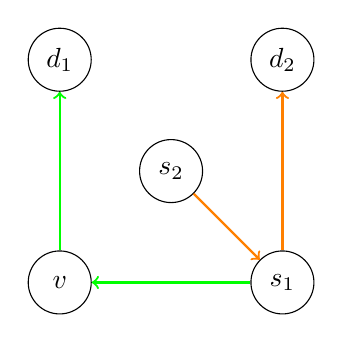
\begin{tikzpicture}[node distance={20mm},main/.style = {draw, circle,minimum size=8mm}]
            \node[main] (s2)  {$s_2$};
            \node[main] (d1) [above left of=s2]  {$d_1$};
            \node[main] (d2) [above right of=s2] {$d_2$};
            \node[main] (v)  [below left of=s2] {$v$};
            \node[main] (s1) [below right of=s2] {$s_1$};
            \draw [->,green,thick] (s1) -- (v);
            \draw [->,green,thick] (v) -- (d1);
            \draw [->,orange,thick] (s2) -- (s1);
            \draw [->,orange,thick] (s1) -- (d2);

        \end{tikzpicture}
        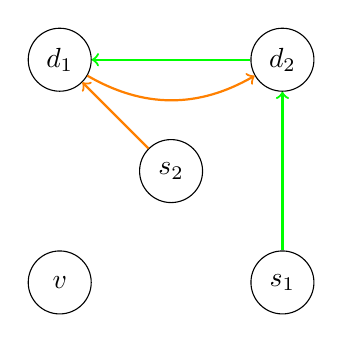
\begin{tikzpicture}[node distance={20mm},main/.style = {draw, circle,minimum size=8mm}]
            \node[main] (s2)  {$s_2$};
            \node[main] (d1) [above left of=s2]  {$d_1$};
            \node[main] (d2) [above right of=s2] {$d_2$};
            \node[main] (v)  [below left of=s2] {$v$};
            \node[main] (s1) [below right of=s2] {$s_1$};
            \draw [->,green,thick] (s1) -- (d2);
            \draw [->,green,thick] (d2) -- (d1);
            \draw [->,orange,thick] (s2) -- (d1);
            \draw [->,orange,thick] (d1) edge[bend right] (d2);

        \end{tikzpicture}
    \end{center}
    Property:
    \begin{itemize}
        \item Property: avoid congestion on the link $s_1-d_2$ 
    \end{itemize}
    Current Behavior:
    \begin{enumerate}
        \item Migrate the green path
    \end{enumerate}
\end{frame}

\begin{frame}
    \begin{center}
        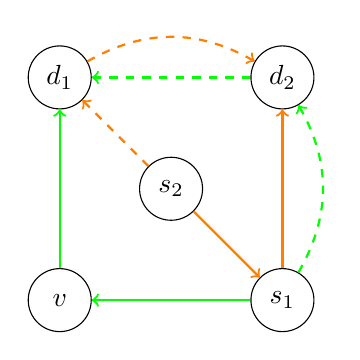
\begin{tikzpicture}[node distance={20mm},main/.style = {draw, circle,minimum size=8mm}]
            \node[main] (s2)  {$s_2$};
            \node[main] (d1) [above left of=s2]  {$d_1$};
            \node[main] (d2) [above right of=s2] {$d_2$};
            \node[main] (v)  [below left of=s2] {$v$};
            \node[main] (s1) [below right of=s2] {$s_1$};
            \draw [->,green,thick] (s1) -- (v);
            \draw [->,green,thick] (v) -- (d1);
            \draw [->,orange,thick] (s2) -- (s1);
            \draw [->,orange,thick] (s1) -- (d2);

            \draw [->,green,thick,dashed] (s1) edge[bend right] (d2);
            \draw [->,green,thick,dashed] (d2) -- (d1);
            \draw [->,orange,thick,dashed] (s2) -- (d1);
            \draw [->,orange,thick,dashed] (d1) edge[bend left] (d2);
            % \draw [->,green,dashed] (v) -- (d1);
            % \draw [->,orange,dashed] (s2) -- (s1);
            % \draw [->,orange,dashed] (s1) -- (d2);

        \end{tikzpicture}
        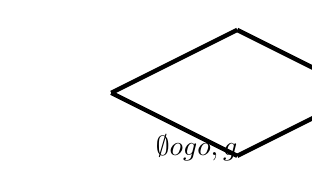
\begin{tikzpicture}[scale=0.8]
            \crd{0}{0}{$\emptyset$}
            \crd[left]{-2}{1}{$\s{o}$}
            \crd[right]{2}{1}{$\s{g}$}
            \crd[right]{0}{2}{$\s{o,g}$}
            \draw [ultra thick] (0,0) -- (2,1);
            \draw [ultra thick] (0,0) -- (-2,1);
            \draw [ultra thick] (-2,1) -- (0,2);
            \draw [ultra thick] (2,1) -- (0,2);
        \end{tikzpicture}
    \end{center}
    Events:
    \begin{itemize}
        \item $g$: migrating the green path 
        \item $o$: migrating the orange path 
    \end{itemize}
    Counterexample:
    \begin{enumerate}
        \item $\sigma = \s{g}$
    \end{enumerate}
\end{frame}

\begin{frame}
    \begin{center}
        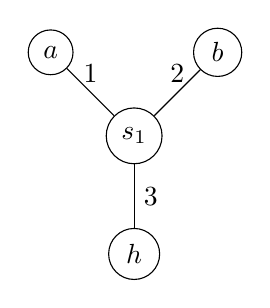
\begin{tikzpicture}[node distance={15mm},main/.style = {draw, circle}]
            \node[main] (s) {$s_1$};
            \node[main] (h) [below of=s] {$h$};
            \node[main] (a) [above left of=s]{$a$};
            \node[main] (b) [above right of=s]{$b$};
            \draw (a) --  node[above]{1}(s);
            \draw (b) --  node[above]{2}(s);
            \draw (s) --  node[right]{3}(h);
        \end{tikzpicture}
    \end{center}
    Property:
    \begin{itemize}
        \item at least two packets traversing link 3
    \end{itemize}
    Current Behavior:
    \begin{enumerate}
        \item forwarding a packet from 1 to 3
        \item forwarding a packet from 2 to 3
    \end{enumerate}
\end{frame}

\begin{frame}
    \begin{center}
        \begin{center}
            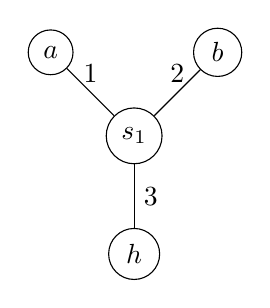
\begin{tikzpicture}[node distance={15mm},main/.style = {draw, circle}]
                \node[main] (s) {$s_1$};
                \node[main] (h) [below of=s] {$h$};
                \node[main] (a) [above left of=s]{$a$};
                \node[main] (b) [above right of=s]{$b$};
                \draw (a) --  node[above]{1}(s);
                \draw (b) --  node[above]{2}(s);
                \draw (s) --  node[right]{3}(h);
            \end{tikzpicture}
        \end{center}
        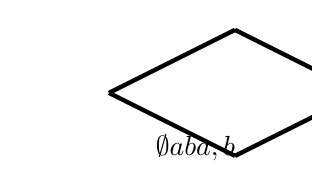
\begin{tikzpicture}[scale=0.8]
            \crd{0}{0}{$\emptyset$}
            \crd[left]{-2}{1}{$\s{a}$}
            \crd[right]{2}{1}{$\s{b}$}
            \crd[right]{0}{2}{$\s{a,b}$}
            \draw [ultra thick] (0,0) -- (2,1);
            \draw [ultra thick] (0,0) -- (-2,1);
            \draw [ultra thick] (-2,1) -- (0,2);
            \draw [ultra thick] (2,1) -- (0,2);
        \end{tikzpicture}
    \end{center}
    Events:
    \begin{itemize}
        \item $a$: Forwarding a packet from 1 to 3
        \item $b$: Forwarding a packet from 2 to 3
    \end{itemize}
    Counterexample: $\sigma = \s{a,b}$
\end{frame}

\begin{frame}
    \begin{center}
        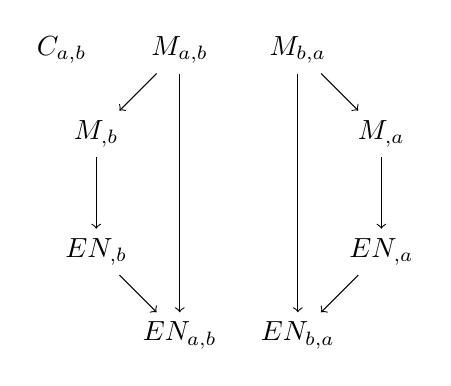
\begin{tikzpicture}[node distance=15mm]
            \node (mab) {$M_{\s{a},b}$};
            \node (mea) [below left of=mab] {$M_{\e,b}$};
            \node (eea) [below of=mea] {$EN_{\e,b}$};
            \node (eab) [below right of=eea]{$EN_{\s{a},b}$};
            \draw[->] (mab) -- (mea);
            \draw[->] (mea) -- (eea);
            \draw[->] (eea) -- (eab);
            \draw[->] (mab) -- (eab);

            \node (mba) [right of=mab] {$M_{\s{b},a}$};
            \node (meb) [below right of=mba] {$M_{\e,a}$};
            \node (eeb) [below of=meb] {$EN_{\e,a}$};
            \node (eba) [below left of=eeb]{$EN_{\s{b},a}$};
            \draw[->] (mba) -- (meb);
            \draw[->] (meb) -- (eeb);
            \draw[->] (eeb) -- (eba);
            \draw[->] (mba) -- (eba);

            \node (cab) [left of=mab] {$C_{a,b}$};

        \end{tikzpicture}
        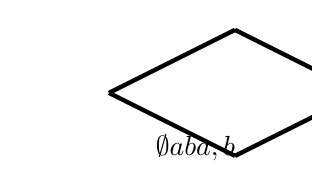
\begin{tikzpicture}[scale=0.8]
            \crd{0}{0}{$\emptyset$}
            \crd[left]{-2}{1}{$\s{a}$}
            \crd[right]{2}{1}{$\s{b}$}
            \crd[right]{0}{2}{$\s{a,b}$}
            \draw [ultra thick] (0,0) -- (2,1);
            \draw [ultra thick] (0,0) -- (-2,1);
            \draw [ultra thick] (-2,1) -- (0,2);
            \draw [ultra thick] (2,1) -- (0,2);
        \end{tikzpicture}
    \end{center}
    \begin{itemize}
        \item Counterexample: $\sigma = \s{a,b}$
        \item Cause: $C(a,b) = \F$
        \item Witness: $(\e,\e, \T)$
    \end{itemize}
\end{frame}

\begin{frame}
    \begin{center}
        \begin{tikzpicture}[node distance=15mm]
            \node[r,label=$\F$] (mab) {$M_{\s{a},b}$};
            \node[g,label=$\T$](mea) [below left of=mab] {$M_{\e,b}$};
            \node[g,label=$\T$](eea) [below of=mea] {$EN_{\e,b}$};
            \node[g,label=$\T$](eab) [below right of=eea]{$EN_{\s{a},b}$};
            \draw[->] (mab) -- (mea);
            \draw[->] (mea) -- (eea);
            \draw[->] (eea) -- (eab);
            \draw[->] (mab) -- (eab);

            \node [r,label=$\F$](mba) [right of=mab] {$M_{\s{b},a}$};
            \node [g,label=$\T$](meb) [below right of=mba] {$M_{\e,a}$};
            \node [g,label=$\T$](eeb) [below of=meb] {$EN_{\e,a}$};
            \node [g,label=$\T$](eba) [below left of=eeb]{$EN_{\s{b},a}$};
            \draw[->] (mba) -- (meb);
            \draw[->] (meb) -- (eeb);
            \draw[->] (eeb) -- (eba);
            \draw[->] (mba) -- (eba);

            \node [r,label=$\F$] (cab) [left of=mab] {$C_{a,b}$};

        \end{tikzpicture}
        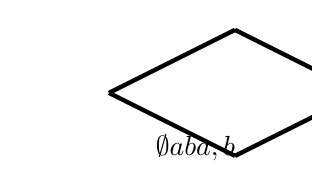
\begin{tikzpicture}[scale=0.8]
            \crd{0}{0}{$\emptyset$}
            \crd[left]{-2}{1}{$\s{a}$}
            \crd[right]{2}{1}{$\s{b}$}
            \crd[right]{0}{2}{$\s{a,b}$}
            \draw [ultra thick] (0,0) -- (2,1);
            \draw [ultra thick] (0,0) -- (-2,1);
            \draw [ultra thick] (-2,1) -- (0,2);
            \draw [ultra thick] (2,1) -- (0,2);
        \end{tikzpicture}
    \end{center}
\end{frame}


\begin{frame}
    \begin{center}
        \begin{tikzpicture}[node distance=15mm]
            \node [r,label=$\F$](mab) {$M_{\s{a},b}$};
            \node[g,label=$\T$](mea)     [below left of=mab] {$M_{\e,b}$};
            \node[g,label=$\T$](eea)    [below of=mea] {$EN_{\e,b}$};
            \node[g,label=$\T$](eab)    [below right of=eea]{$EN_{\s{a},b}$};
            \draw[->] (mab) -- (mea);
            \draw[->] (mea) -- (eea);
            \draw[->] (eea) -- (eab);
            \draw[->] (mab) -- (eab);

            \node [r,label=$\F$](mba) [right of=mab] {$M_{\s{b},a}$};
            \node [g,label=$\T$](meb) [below right of=mba] {$M_{\e,a}$};
            \node [g,label=$\T$](eeb) [below of=meb] {$EN_{\e,a}$};
            \node [g,label=$\T$](eba) [below left of=eeb]{$EN_{\s{b},a}$};
            \draw[->] (mba) -- (meb);
            \draw[->] (meb) -- (eeb);
            \draw[->] (eeb) -- (eba);
            \draw[->] (mba) -- (eba);

            \node [o,label=$\not \F \T$] (cab) [left of=mab] {$C_{a,b}$};

        \end{tikzpicture}
        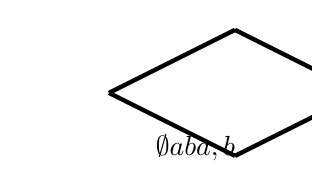
\begin{tikzpicture}[scale=0.8]
            \crd{0}{0}{$\emptyset$}
            \crd[left]{-2}{1}{$\s{a}$}
            \crd[right]{2}{1}{$\s{b}$}
            \crd[right]{0}{2}{$\s{a,b}$}
            \draw [ultra thick] (0,0) -- (2,1);
            \draw [ultra thick] (0,0) -- (-2,1);
            \draw [ultra thick] (-2,1) -- (0,2);
            \draw [ultra thick] (2,1) -- (0,2);
        \end{tikzpicture}
    \end{center}
\end{frame}

\begin{frame}
    \begin{center}
        \begin{tikzpicture}[node distance=15mm]
            \node[r,label=$\F$](mab) {$M_{\s{a},b}$};
            \node[g,label=$\T$](mea)     [below left of=mab] {$M_{\e,b}$};
            \node[g,label=$\T$](eea)    [below of=mea] {$EN_{\e,b}$};
            \node[g,label=$\T$](eab)    [below right of=eea]{$EN_{\s{a},b}$};
            \draw[->] (mab) -- (mea);
            \draw[->] (mea) -- (eea);
            \draw[->] (eea) -- (eab);
            \draw[->] (mab) -- (eab);

            \node [r,label=$\F$](mba) [right of=mab] {$M_{\s{b},a}$};
            \node [g,label=$\T$](meb) [below right of=mba] {$M_{\e,a}$};
            \node [g,label=$\T$](eeb) [below of=meb] {$EN_{\e,a}$};
            \node [g,label=$\T$](eba) [below left of=eeb]{$EN_{\s{b},a}$};
            \draw[->] (mba) -- (meb);
            \draw[->] (meb) -- (eeb);
            \draw[->] (eeb) -- (eba);
            \draw[->] (mba) -- (eba);

            \node [g,label=$\T$] (cab) [left of=mab] {$C_{a,b}$};

        \end{tikzpicture}
        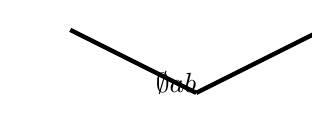
\begin{tikzpicture}[scale=0.8]
            \crd{0}{0}{$\emptyset$}
            \crd[left]{-2}{1}{$\s{a}$}
            \crd[right]{2}{1}{$\s{b}$}
            \draw [ultra thick] (0,0) -- (2,1);
            \draw [ultra thick] (0,0) -- (-2,1);
        \end{tikzpicture}
    \end{center}
\end{frame}